\section{Durchführung}
\label{sec:Durchführung}

\subsection{Versuchsaufbau}
\label{sec:Aufbau}
Wie bereits in Kapitel \ref{sec:nachweis} beschrieben, ist in dem Versuchsaufbau eine evakuierte Photozelle (vgl.Abb.\ref{fig:Photozelle}) mit einem
Picoamperemeter und einer variablen Spannungsquelle verbunden (vgl.Abb.\ref{fig:Schaltung}). Da das Licht, mit welchem die Kathode 
bestrahlt wird, aber eine feste Frequenz $\nu$ besitzen soll, wird auch eine optische Konstuktion benötigt. 
\begin{figure}
    \centering
    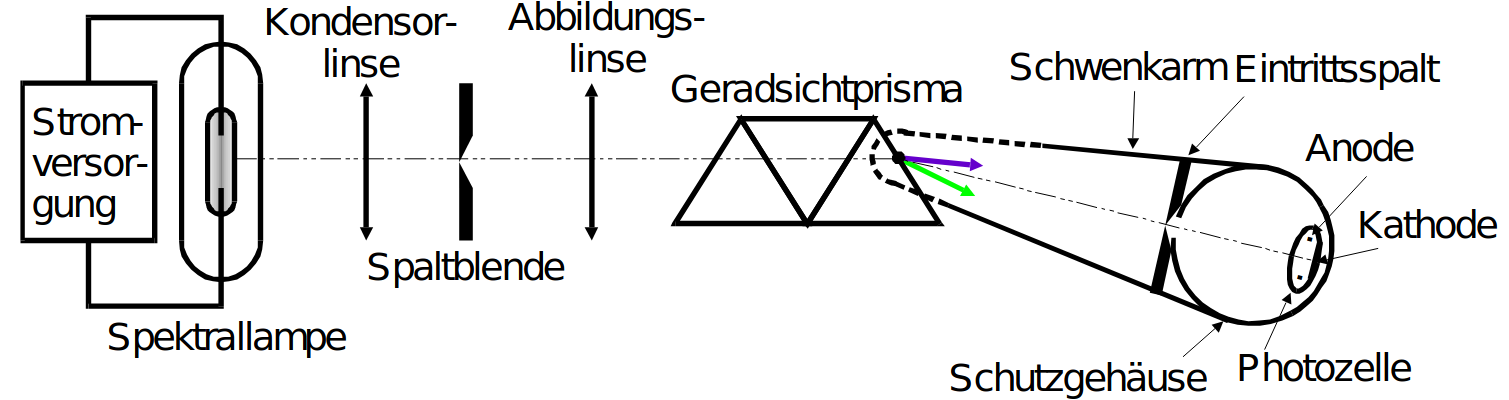
\includegraphics[scale=0.3]{pictures/OptischerTeil.png}
    \caption{Optische Konstruktion zur Gewinnung monochromatischen Lichts. \cite{AP01}}
    \label{fig:optisch}
\end{figure}
Wie in Abbildung \ref{fig:optisch} zu sehen, wird von einer 
Spektrallampe ausgesendetes polychromatisches Licht durch Linsen und einen Spalt fokosiert und dann mit einem Prisma in seine monochromatischen
Spaktrallinien zerlegt. Die Photozelle kann jetzt so auf einem Schwenkarm bewegt werden, dass immer nur eine Spektrallinie ais die Kathode
fällt. Somit können für mehrere Lichtfrequenzen Messungen durchgeführt werden. 

\subsection{Ausmessung des Photostroms}
\label{sec:ausmessen}
Vor Begin der Messung muss der Dunkelstrom gemessen werden, welches das Picoamperemeter auch ohne Anschalten der Lampe anzeigt. Erst dann 
wird die Spektrallampe angeschaltet. Nach Ausrichten einer Spektrallinie wird die Spannung von $\SI{2}{\volt}$ bis $\SI{-2}{\volt}$ in 
$\SI{0.2}{\volt}$-Schritten variiert. Dabei werden die gemessenen Spannungen abgelesen und notiert. Diese Messung erfolgt für die 
die grüne ($\lambda=\SI{546}{\nano\metre}$), die blaugrüne ($\lambda=\SI{492}{\nano\metre}$) und die zweite violette 
($\lambda=\SI{408}{\nano\metre}$) Spektrallinie. 
\\\noindent
Für die gelbe Spektrallinie ($\lambda=\SI{579}{\nano\metre}$) wird die Spannung in einem Bereich von $\SI{20}{\volt}$ bis $\SI{-2}{\volt}$
variiert, wobei in dem Bereich von $\SI{20}{\volt}$ bis $\SI{2}{\volt}$ eine Schrittweite von $\SI{1}{\volt}$ gewählt wird. 